%!TEX root = ../report.tex

\section{Ausdauer}
Definition: Ermüdungswiderstandsfähigkeit (konditionell und informationell) und Regenerationsfähigkeit

\subsection{Systematik}
\subsubsection{Belastungsdauer}
\begin{itemize}
  \item Kurzzeitausdauer (<35s)
  \item Mittelzeit-Ausdauer(35s - 8min)
  \item Langzeitausdauer (> 8min): LZA I: 8-30min, LZA II: 30min - 3h, LZA III: 3-9h, LZA IV: >9h
\end{itemize}

\subsubsection{Allgemeine vs spezielle Ausdauer}
\begin{itemize}
  \item Allgemeine Ausdauer: Grundlage für Regeneration, Training und Erholung und Voraussetzung für spezielles Training
  \item Spezielle Ausdauer: Wettkampfspezifische Ausdauer-Anforderungen (wichtiger für sportlichen Erfolg)
\end{itemize}

\paragraph{KsA: Koeffizient der speziellen Ausdauer}
= durchschnittliche 100m-Zeit obere Nachbarstrecke / durchschnittliche 100m-Zeit untere Nachbarstrecke

\subsection{Energiebereitstellung}
\paragraph{Mechanismen}
\begin{itemize}
  \item Systematik: Je nach Dauer und Intensität der Belastung wird Energie aus verschiedenen Substanzen gewonnen.
  \item Energiegewinnung aus Substrat:
    \begin{itemize}
      \item Energiefluss: Rate, mit der Energie zur Verfügung gestellt werden kann.
      \item Kapazität: Energievorrat
    \end{itemize}
  \item Problem: Maximale Energie nur kurzfristig verfügbar\\
    Dauerleistungsgrenze: ca 40%
  \item Energiearten
    \begin{itemize}
      \item alaktazid
      \item laktazid
      \item aerob
    \end{itemize}
\end{itemize}

\subsection{Determinaten der Ausdauer}
\begin{centering}
\begin{tabular}{m{0.2\textwidth} | m{0.3\textwidth} | m{0.3\textwidth}}
                          & Intensiv                                                         & Extensiv \\ \hline
     Energiespeicher      & Phosphat                                                         & Glykogen \\ \hline                          
     Enzymaktivityät      & Phosphatstoffwechsel Laktatabbau und -toleranz                   & Kohlenhydrat- und Fettstoffwechsel \\ \hline
     Muskulatur           & vortriebrelevante Muskulatur                                     & Haltearbeit verrichtete Muskulatur \\ \hline
     Sauerstoffversorgung & Schlagvolumen, Kapillarisierung der Arbeitsmuskulatur, Blutmenge \\ \hline
     Qualität der Technik & Bewegungsökonomie \\ \hline                                               
     Psychische Eigensch. & Durchhaltevermögen, "Stehvermögen", "mentale Härte" \\
\end{tabular}
\end{centering}

\subsection{Herz-Kreislauf}
\begin{itemize}
  \item Maximale Sauerstoffaufnahme - Normale Werte: 38-42 ml O2/(min x kg) (Frauen) und 44-50 ml O2/(min x kg) \\
    Spitzensportler: ca doppelte Werte
  \item Herzminutenvolumen (abhängig von Herzvolumen und Belastungsherzfrequenz)
    \begin{itemize}
      \item untrainiert: 20 l/min
      \item trainiert: 40 l/min
    \end{itemize}
  \item Blut (abhängig von Blutmenge und Sauerstoffbindungsfähigkeit)
\end{itemize}

\subsection{Methoden nach Trainingsbereichen}
\begin{centering}
\begin{tabular}{m{0.2\textwidth} | m{0.3\textwidth} | m{0.3\textwidth}}
   Trainingsbereich              & Primäres Ziel                                                                   & Methode \\ \hline
   Regeneration                  & Regenerationsbeschleunigung                                                     & Extensive Dauermethode \\ \hline
   Grundlagenausdauer 1          & Ausdauerfähigkeit niedriger Intensitätsbereich                                  & Intensive Dauermethode \\ \hline
   Grundlagenausdauer 2          & Ausdauerfähigkeit hoher Intensitätsbereich und physiol. Kapazitätserweiterungen & Intervallmethoden \\ \hline
   Wettkampfspezifische Ausdauer & Ausdauerfähigkeit im Wettkampfbereich                                           & Wettkampfmethode \\     
\end{tabular}
\end{centering}

\subsection{Belastungsmotive und Ausdauertraining}
\begin{itemize}
  \item Intensität: Stärke eines Einzelreizes
  \item Dauer: Wirkungsdauer eines Einzelreizes
  \item Umfang: Dauer \& Zahl der Reize/Trainingseinheit
  \item Dichte: Zeitliches Verhältnis zwischen Belastungs- und Erholungsphasen
  \item Häufigkeit: Zahl der Trainingseinheiten pro Trainingszeitraum
\end{itemize}

\subsection{Methoden im Überblick}
\begin{itemize}
  \item Dauermethode: Ununterbrochene Dauerbelastung mit geringer intensität und keinen Pausen
    \begin{itemize}
      \item Extensiv: Intensität unterhalb der AS (?) \& Dauer von 20-60min oder mehr.\\ 
        Intension: Rechtsverschiebung der AS, Hoher Energieverbrauch, Regeneration, Gewöhnung an Belastungsmonotonie \\
        \begin{figure}[H]
          \centering
          \begin{subfigure}[b]{0.4\textwidth}
            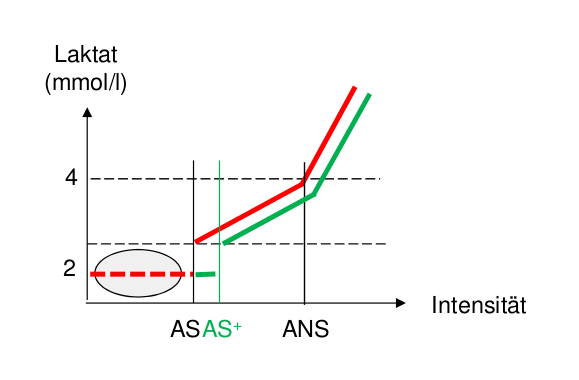
\includegraphics[width=\textwidth]{pictures/dauertraining_extensiv.png}
            \caption{Dauertraining extensiv}
          \end{subfigure}
          \begin{subfigure}[b]{0.4\textwidth}
            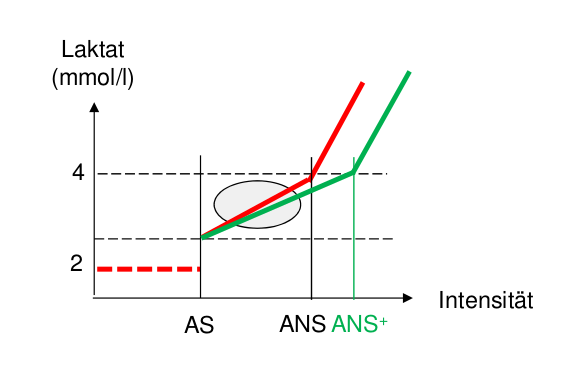
\includegraphics[width=\textwidth]{pictures/dauertraining_intensiv.png}
            \caption{Dauertraining intensiv}
          \end{subfigure}
        \end{figure}
      \item Intensiv: Intensität knapp unterhalb der ANS, Dauer \& Intensität hoch ($\leq$ ED)\\
        Intention: Rechtsverschiebung der ANS, Verbesserung des Glykose- und Laktatabbaus, Laktattoleranz (``MENTALE HÄRTE BITCH'')
    \end{itemize}
  \item Intervallmethoden: Intensität wechselnd über und unter dem ANS, durch Erholungspausen höhere Intensitäten als bei Dauermethoden mgl \\
    Intention: Verbesserung der Leistungsfähigkeit oberhalb der ANS, Phosphatstoffwechsel, hyperthrophie Herzmuskel (Belastungsphase), Erhöhung des Schlagvolumens
    \begin{figure}[H]
      \centering
      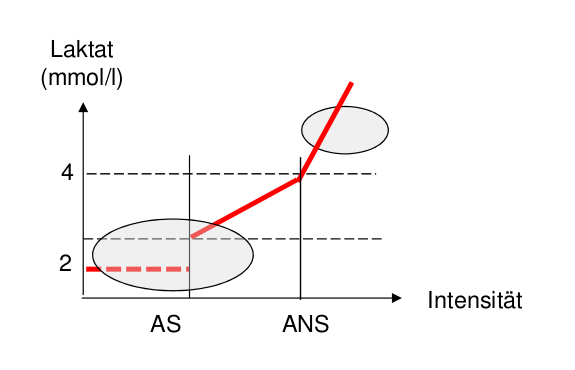
\includegraphics[width=.5\textwidth]{pictures/intervalltraining.png}
      \caption{Intervallmethoden}
    \end{figure}
\end{itemize}
